\chapter{Developing Tellervo Server}
\index{Developing|(}
\index{Developing!Webservice}
\index{Webservice!Developing}

The Tellervo server is made up of a PHP webservice run by Apache, connecting to a PostgreSQL database.  

The Tellervo webservice is written entirely in PHP.  Like the Desktop Client, the server is developed with Eclipse so most of the setup steps are identical (see chapter \ref{txt:devDesktop}).  You will, however, probably want to install the PHP development plugin so that you get syntax highlighting etc.  See the Eclipse PDT website (\url{http://www.eclipse.org/pdt/}) for further information.


\section{Webservice}

Before making any changes to the webservice you will need to understand its architecture first.  Chapter \ref{txt:webserviceSpec} contains details of the communications specification.

\subsection{Creating new series}

Due to the complications arising from the virtual measurement concept, creating new series in Tellervo is necessarily more complicated than any other of the TRiDaS entities.  The workflow required to create a new series is illustrated in figure \ref{fig:creatingNewMSeries}.

\begin{figure}[hbtp]
  \centering
  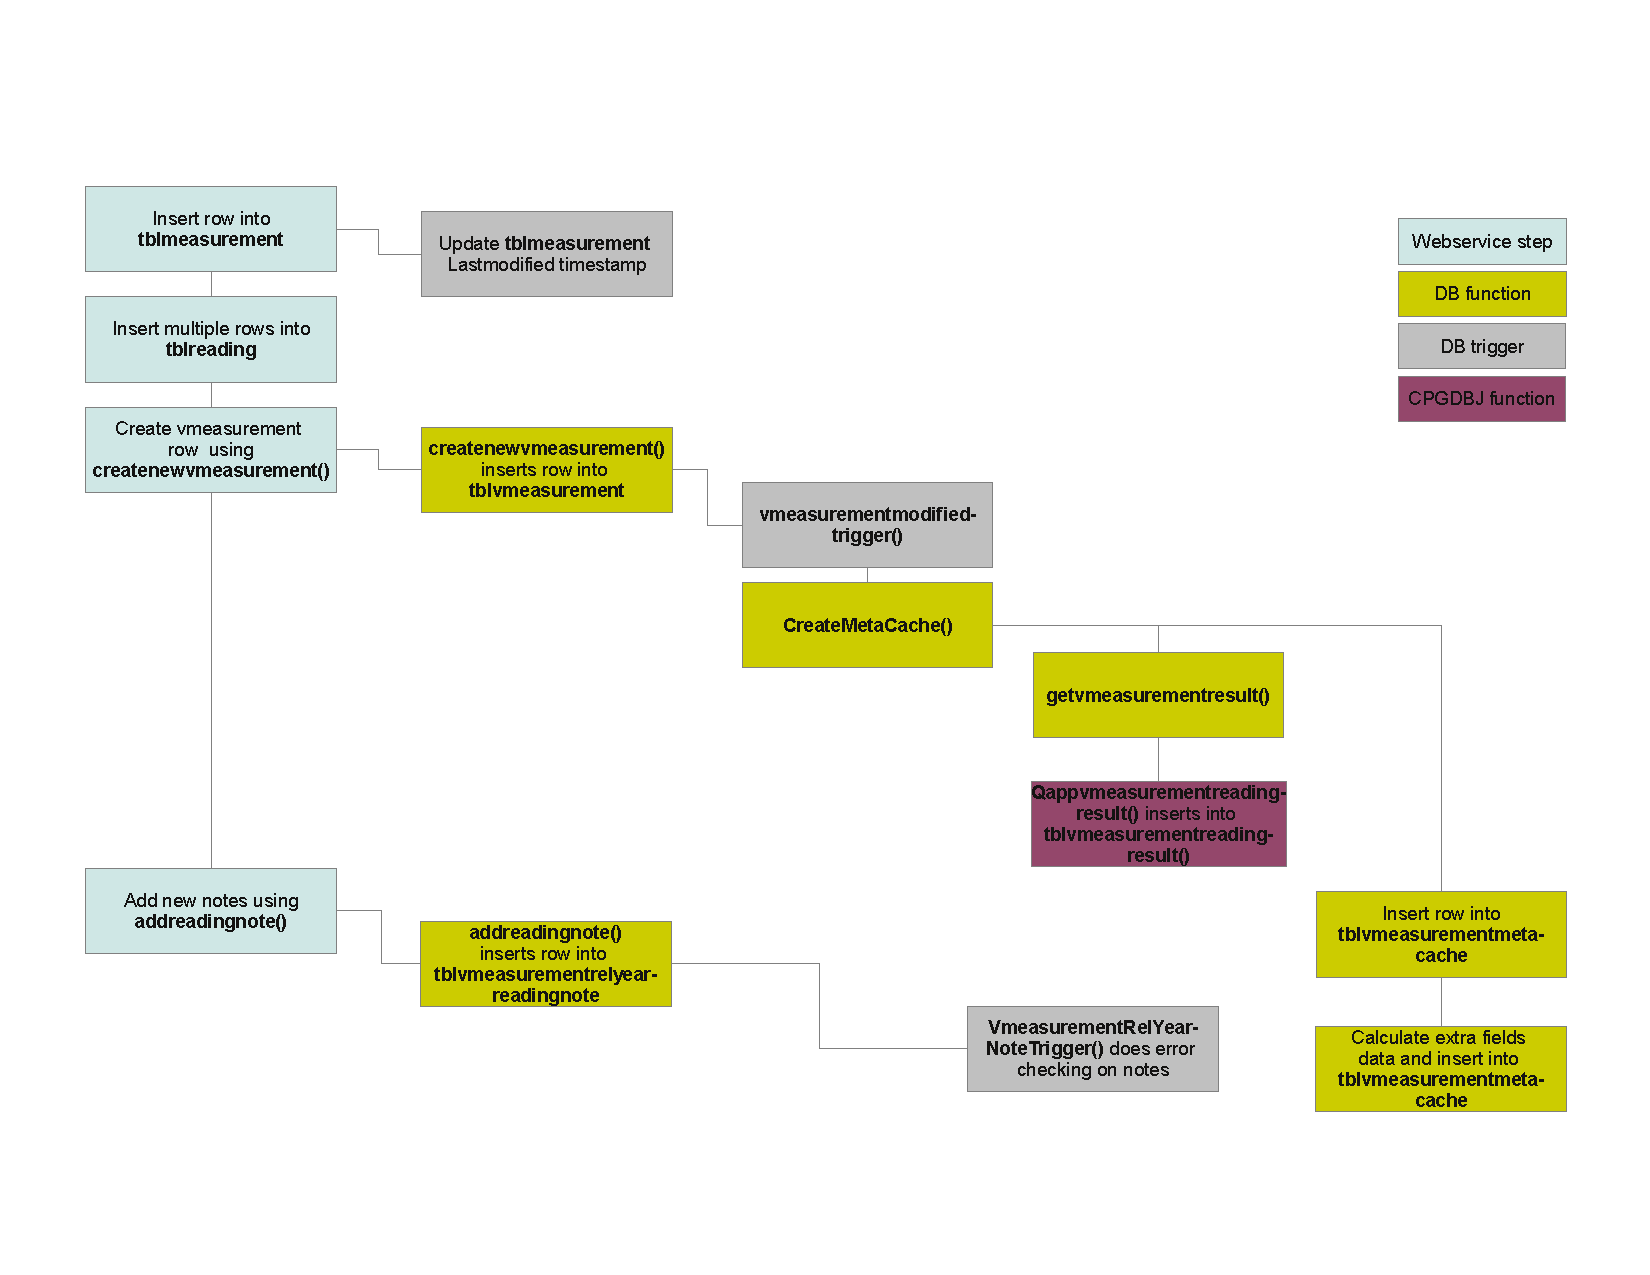
\includegraphics[width=0.8\textwidth]{Images/CreatingNewMSeriesWorkflow.pdf}
  \caption{Illustration of the steps that happen during the creation of a new measurement series. The stages are presented top to bottom in the approximate order in which they are executed.  The majority of the processing is done as a result of the database function createnewvmeasurement() being called by the webservice.}
  \label{fig:creatingNewMSeries}
\end{figure}

\begin{figure}[hbtp]
  \centering
  %\includegraphics[width=0.8\textwidth]{Images/EditingMSeriesWorkflow.pdf}
  \caption{Illustration of the steps that happen during the alteration of an existing measurement series. The stages are presented top to bottom in the approximate order in which they are executed.}
  \label{fig:editingNewMSeries}
\end{figure}

\begin{figure}[hbtp]
  \centering
  \includegraphics[width=0.8\textwidth]{Images/CreatingNewDSeriesWorkflow.pdf}
  \caption{Illustration of the steps that happen during the creation of a new derived series. The stages are presented top to bottom in the approximate order in which they are executed.  Depending on the type of derived series being created, a different database function is called to finish the new vmeasurement.}
  \label{fig:creatingNewMSeries}
\end{figure}

\begin{figure}[hbtp]
  \centering
  %\includegraphics[width=0.8\textwidth]{Images/EditingDSeriesWorkflow.pdf}
  \caption{Illustration of the steps that happen during the alteration of an existing derived series. The stages are presented top to bottom in the approximate order in which they are executed. Note that presently it is not possible to alter the parameters of a derived series.}
  \label{fig:editingNewMSeries}
\end{figure}



\section{Server package}
\label{txt:serverPackage}
\index{Packaging!Server}
The Ubuntu server package is built by Maven at the same time as the desktop package (see section \ref{txt:buildScript}) during the package goal.  

The server packaging is done as a secondary execution of the JDeb plugin.  JDeb is configured in the pom.xml by including all the files that need to be copied along with where in the target file system they should be placed. The database files are installed to `/usr/share/tellervo-server' and the webservices files to `/var/www/tellervo/'. 

The metadata for the deb file is included in the control file located in Native/BuildResources/LinBuild/ServerControl.  JDeb makes use of Ubuntu's excellent package management system to handle the dependencies.  Adding or editing dependencies is simply a matter of changing the `depends' attribute control file.  

The ServerControl folder also contains scripts called preinst, postinst, prerm and postrm, which are launched before and after installation, and before uninstalling.  These files are called with different parameters depending on whether this is part of a fresh install, an upgrade, or an aborted install.  There are a number of rules that the resulting deb package should follow (e.g.\ if a program is configured twice, then the second run should know and understand about previously provided details), the details of which can be found in the Debian Policy Manual\footnote{Debian Policy Manual -- \url{http://www.debian.org/doc/debian-policy/} but a more accessible description is found at \url{http://wiki.debian.org/MaintainerScripts}}, along with information how and when each of the pre and post scripts is run.  Hopefully this side of the server packaging will not need to be touched again, but if you are making changes and are doing anything more than simple tweaks, please consult the Debian policy documentation.

If changes are required, figure \ref{fig:debflowchart} highlights the order that the pre and post scripts are run and with what parameters.  


\begin{figure}[p]
  \centering
  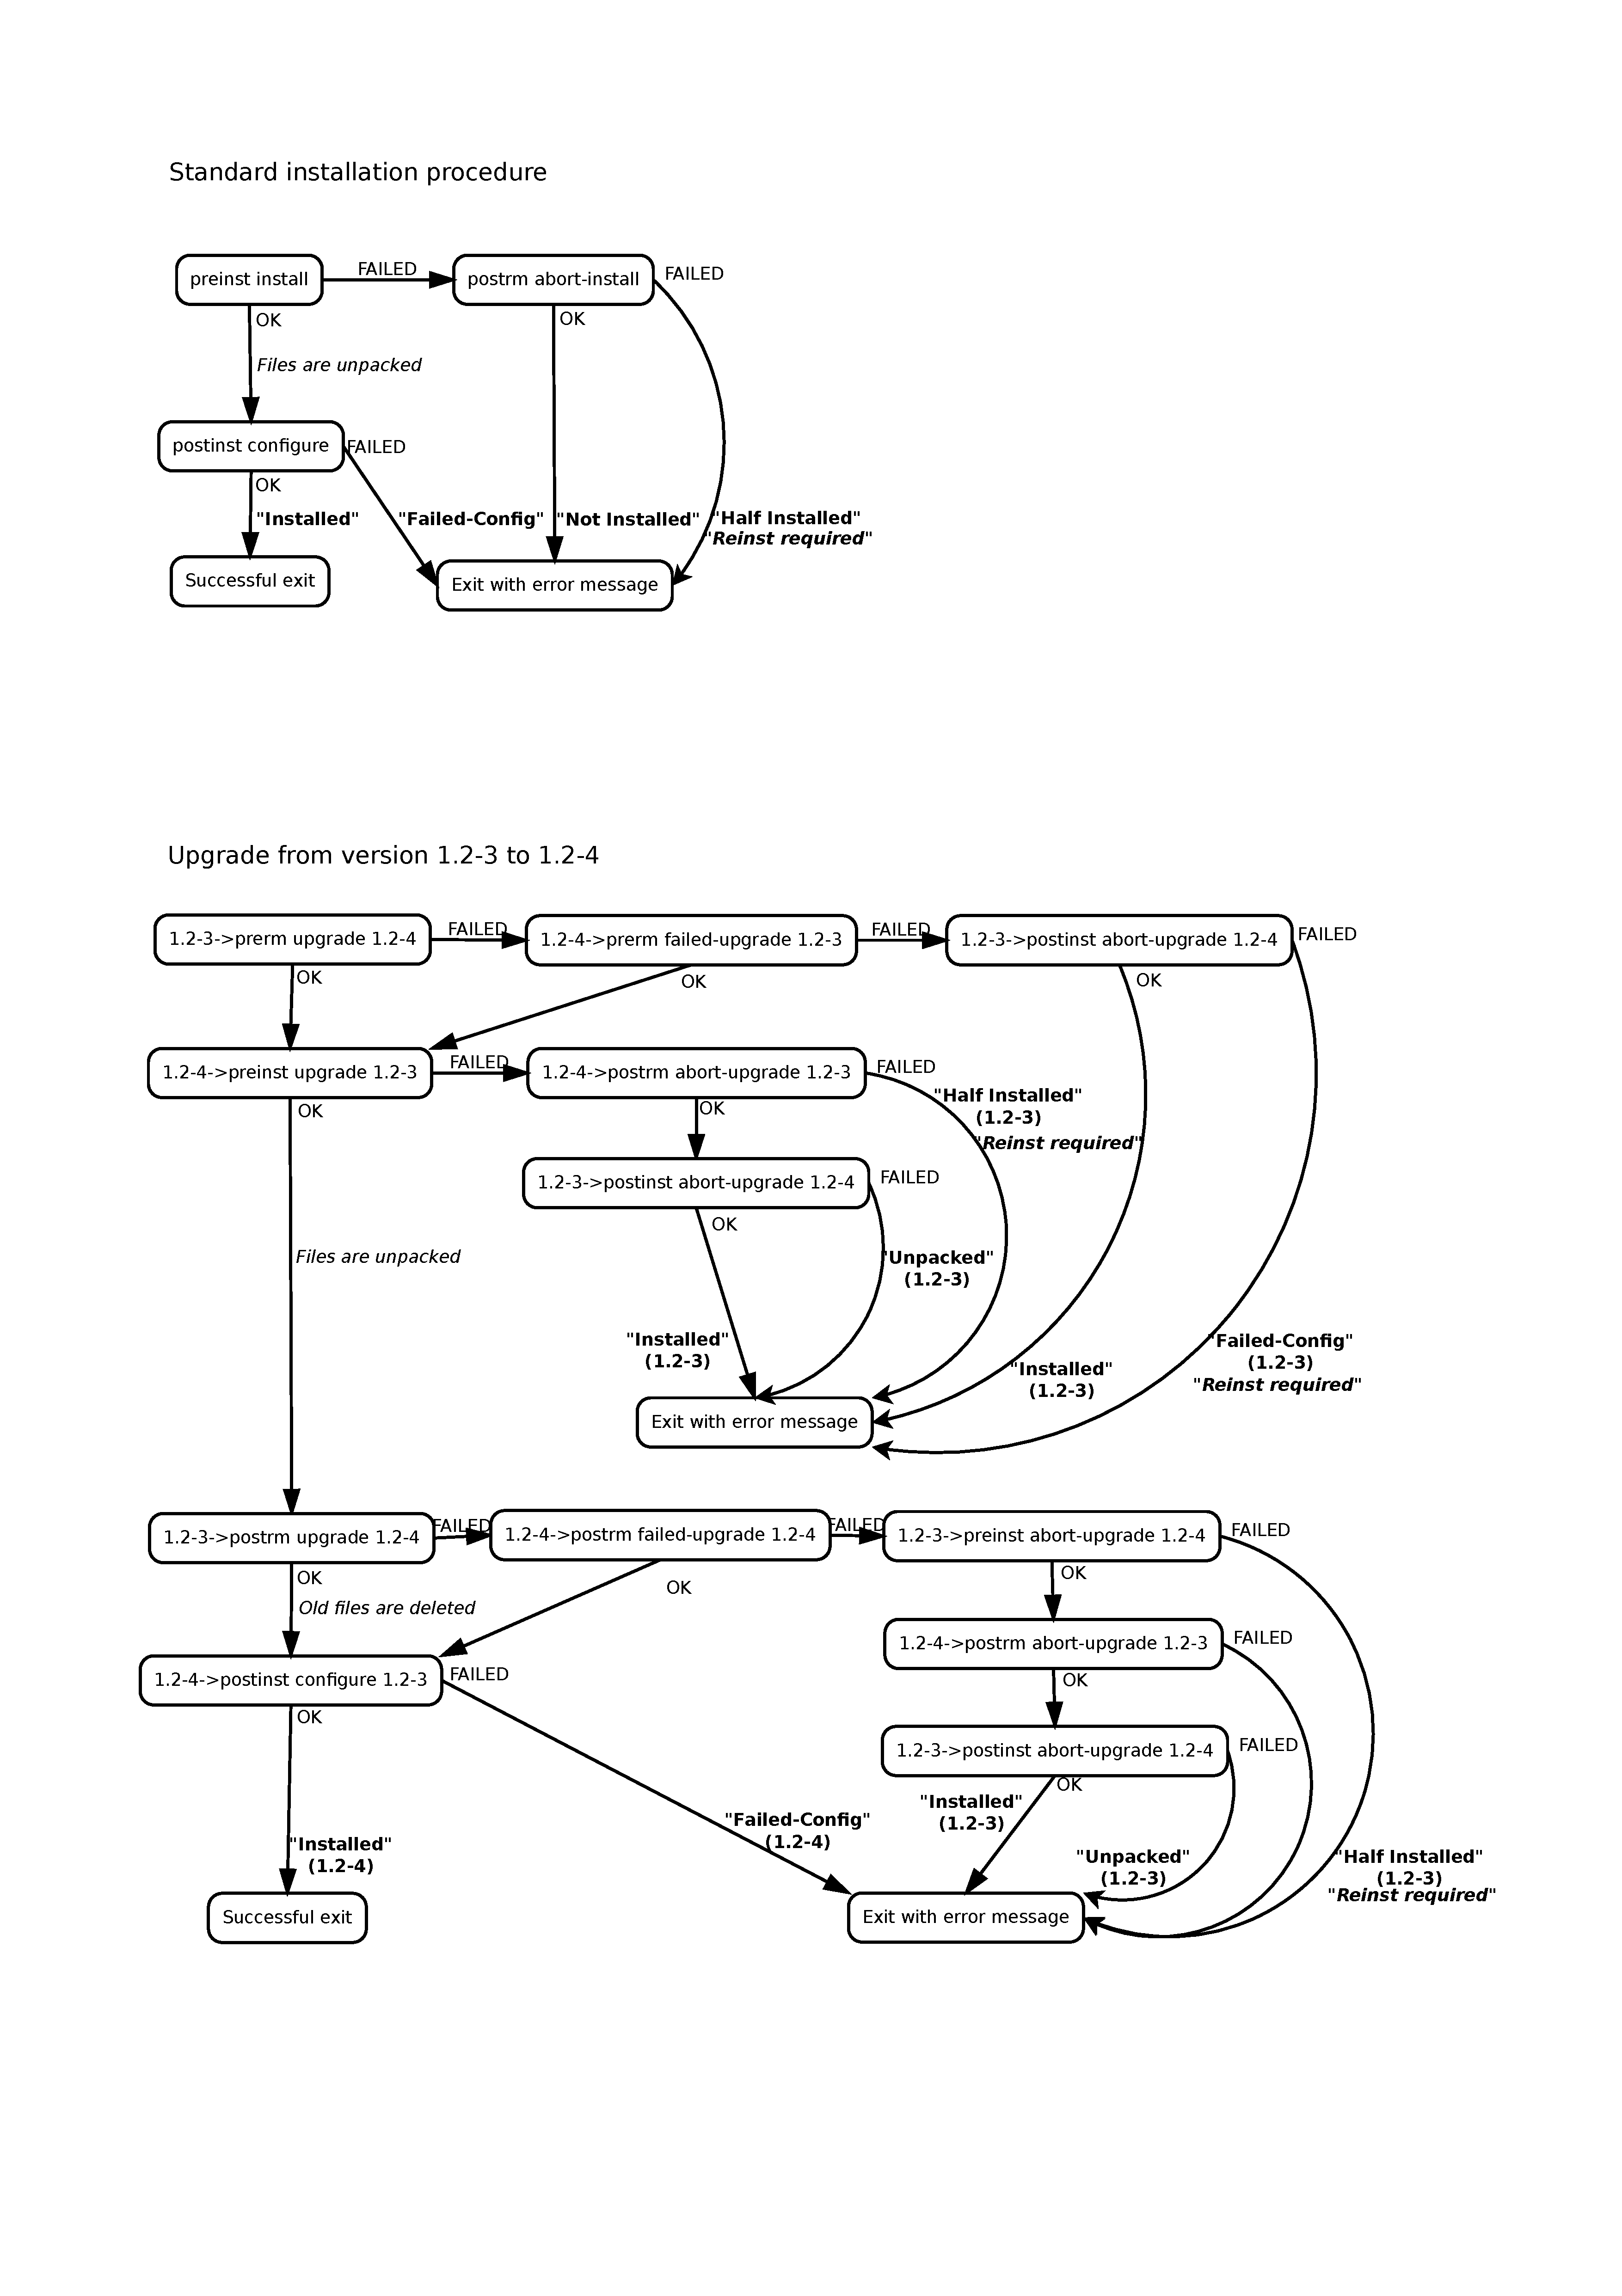
\includegraphics[width=\textwidth]{Images/install-and-upgrade-procedure.pdf}
  \caption{Flow chart showing how the prerm, preinst, postrm, postinst scripts are run along with the parameters passed to them when installing and upgrading.  }
  \label{fig:debflowchart}
\end{figure}

The postinst script is used to trigger the interactive script that helps the user configure the Tellervo server (described further in section \ref{txt:tellervo-server-script}).  The steps are as follows:  

\begin{itemize*}
 \item Check the user running the script is root as we're doing privileged functions
 \item Generated scripts from templates
 \item Configure PostgreSQL database, creating users and/or database if requested otherwise obtaining details if they already exist
 \item Configure PostgreSQL to allow access to the specified database user
 \item Configure Apache to access the webservice
 \item Verify setup by checking Apache and PostgreSQL are running, that the webservice is accessible, the database is accessible and that various configuration files can be read
 \item Print test report to screen
\end{itemize*}

\subsection{Tellervo server script}
\label{txt:tellervo-server-script}

At the heart of most of the configuration and control of the Tellervo server is the tellervo-server script.  This is a command line PHP script that is launched after installation and can be re-run by the user to make changes to the configuration.  Although such a script would normally be written in Bash or similar, we decided to go with PHP because of the requirement to interact with the Tellervo PostgreSQL database.  

The script isolates the common tasks performed into functions.  It uses the getopt() function to read both long (e.g. --blah) and short (e.g. -b) arguments from the command line.  These depending on the arguments given, the script then calls the relevant functions.

To comply with standard protocols, the script uses the exit() function to return whether the requested task was successful or not.  Returning zero means the script was successful, and returning any other integer means the script failed.  This is important so that the package management system knows when things have gone wrong, and can then attempt to roll back if possible.

The script includes a number of helper functions and classes that you may find useful when modifying the script:

\begin{description}
 \item[echoTruncatedString(\$str, \$length] -- echos a string to the console but truncates it to \$length if necessary.  If the string is shorter than \$length, then it is padded with spaces.  This is useful to ensure the following text is displayed aligned, e.g. test results.
 \item[requireRoot()] -- check whether the user running the script has root privileges.
 \item[checkServiceIsRunning(\$service)] -- checks whether the named service is running on the system.  This is performed by checking whether the provided string is present in the response from the shell command `ps ax'.
 \item[setConfigVariable(\$var, \$value)] -- does a search and replace for a placeholder variable in the config.php file, replacing with \$value.  Placeholders should be stored in the config.php template as \verb|%%VARIABLENAME%%|.
 \item[promptForPwd(\$isCreating=TRUE)] -- is an interactive script for getting a password from the user.  It checks that the password
 is strong and asks for it twice to check for typos. 
 \item[class Colors] -- can be used to display coloured text on the console.  Useful for highlighting errors and test results.

\end{description}

\section{Handling version dependencies}
In an ideal world, the API for how clients talk to the Tellervo server would never change.  Unfortunately, we don't live in an ideal world!  New features in Tellervo will require changes to the API, as will changes to TRiDaS.  In anticipation of such changes, the Tellervo server includes a mechanism for detecting when a client is too old to handle the API that it is using.  In this case the server will refuse to handle the request.  A similar complementary mechanism is in place in the client for instances when a client is attempting to talk to an older server that it no longer supports.  

At the moment, the Tellervo desktop client is the only known software that talks to the Tellervo server, but in the future we may have other 3rd party clients making requests.  For example it would be possible to develop a central data repository (much like the ITRDB or perhaps as an extension to the existing ITRDB) that harvests data from multiple labs each running the Tellervo server. Alternatively, existing 3rd party desktop applications (e.g. TSAP-Win, PAST4 etc) may be extended to enable them to obtain data directly from servers running the Tellervo server software.  Either way, it is important to include the ability to specify the oldest versions of clients that are able to connect, and also to be able to specify different versions for different types of clients. 

It is also necessary to include the ability to allow or disallow access to the server by unknown client applications.  If a new program is written by other developers and it attempts to access the server it could contain bugs (or even malicious code\footnote{Keep in mind though that a user with the necessary privileges would need to provide this new program with their credentials for it to make changes to data.}) that interferes with the server.  For a production instance of the server this is obviously undesirable, therefore the systems configuration option `onlyAllowKnownClients' is set to TRUE.  

\subsection{Client requiring a recent server}

In the event that changes are made to the client that means it needs a particular version of the server to run, then this information is specified in the static string App.earliestServerVersionSupported.  This value should be a three part version number e.g.\ 1.1.1.  No other changes are required.  When the user tries to connect to a server with a version prior to the minimum version specified, they will be shown an error message explaining that they need to get the Tellervo administrator to upgrade the server.  

\subsection{Server requires a recent client}

In the event that changes are made to the server which mean that a recent version of the client is required, then this information is stored in the database in the tblsupportedclient table.  The `client' field should contain a unique portion of the HTTP\_USER\_AGENT header provided by the client.  The version number field should be a 2 or 3 part number e.g.\ 1.1 or 1.1.1.  In the event that a user tried to connect to a Tellervo server using a client that is too old, then they will be given a clear error message informing them that they need to upgrade.


\section{Handling server configuration}
\index{systemconfig.php}
\index{config.php}
The Tellervo server is configured using two main PHP files: config.php and systemconfig.php.  The configuration is split into two primarily because the config.php values are considered to be editable by the server administrator, whereas those in systemconfig.php should normally only be edited by Tellervo developers.  

If you want to make configuration options editable by the administrator of the Tellervo server, then these should be implemented within the config.php file.  There is a config.php.template file which is used to construct the config.php file on the users system.  Simply adding hardcoded entries to this file is the simplest way when a default value is appropriate.  If the value of your field needs to be generated either by asking the administrator a question (e.g. name of lab), or dynamically at the time of installation (e.g. IP address of the server) then this template file should contain placeholder values which can then be replaced by the tellervo-server configuration script.  For instance the config.php.template file contains a placeholder for the hostname of the server like this: \verb|$hostname = "%%IP%%";|.  The value is set by the tellervo-server script using the function \verb|setConfigVariable($var, $value)|.  Keep in mind though, that during an upgrade, the config.php is maintained and not replaced.  If you make additions to the config.php.template you will also need to make provision for handling changes to the end users existing config.php.

If you want to add new configuration fields that don't need to be edited by the system administrator, these should be handled in the systemconfig.php file.  The systemconfig.php file is automatically generated during installation/upgrade of the server from entries in the database table tblconfig.  This means that any changes to the system configuration can be handled as part of the database upgrade simply by adding new rows or editing existing rows in tblconfig.  Each entry in this table is made available to the webservice as a global variable once the tellervo-server script has been run.  For instance the row containing key=wsversion and value=1.0.0 is available as the variable \$wsversion within the webservice. 



\section{Making a new release}

As mentioned in section \ref{txt:serverPackage}, the server package is created at the same time as the desktop binaries as part of the Maven package procedure.  There are, however, a number of steps you need to undertake to make sure this goes smoothly.

\begin{itemize}
 \item Make sure this documentation is up-to-date! 
 \item Increment the \verb|<serverversion>| tag in the pom.xml file
 \item Make sure that any upgrades that need to be made to the database are included in a new and unique SQL file stored in Databases/db-upgrade-patches.  Each file from this folder is run by the installer unless it has previously been run.  
 \item If this version of the server needs a particular version of the client then you'll need to set this value in the tblsupportedclient table by including a relevant SQL statement in your db-update-patches script e.g.: \code{UPDATE tblsupportedclient SET minversion='2.13' WHERE client='Tellervo WSI';}
 \item Run maven package to produce the server deb file.
 \item Create a clean Ubuntu VirtualBox installation with the user `tellervo' and the password `dendrochronology'
 \item Install the deb file and dependencies as normal, configuring the server with temporary settings
 \item Run \verb|sudo tellervo-server --deploy| to remove the temporary settings and set up ready for users first run
 \item Shutdown the virtual appliance then export.  Add in all the metadata as required.
 \item Copy the virtual appliance file and the native deb file to the web server for release.  The server PHP code will automatically pick up the extra files and offer them to users.  
 \item Update the download/index.php file to reflect the `preferred' version choice for users.
 \item TEST!  If users are running this as an upgrade, then we need to ensure this goes smoothly.  Although they are told to backup their database before running we should assume they've ignored the warning and that we are altering precious data. Test both a fresh install and an upgrade from the previous version.
\end{itemize}



\section{Administering the Maven repository}
The following information is only necessary for the lead-developer and outlines the steps necessary to install and maintain the central Maven repository for Tellervo.  This Maven repository should provide all other developers with the libraries required to develop Tellervo and which are bundled in the release packages.

The repository tool that we currently use is Apache Archiva.  Installation is relatively simple:

\begin{enumerate}
 \item Download the zip bundle from the Apache Archiva website
 \item Unzip and place on the server in a suitable location (e.g.\ usr/share/apache-archiva)
 \item Run `sudo bin/archiva start'
\end{enumerate}

If you have an existing backup of the Archiva database then you can place this in the data folder and you should be good to go.  If not you will need to do the following steps to configure the repository from scratch:

\begin{enumerate}
 \item Go to `http://www.tridas.org:8080/archiva/' in your web browser and set up the admin account.  If you're setting this up on another domain remember you'll need to change the repository URLs in both the distributionManagement and repositories sections of your pom file
 \item In the repositories tab you need to configure both releases and snapshot repositories
 \item Set up users with `Repository Manager' permissions for each user that would like to deploy to the repository.  They will need to configure their .m2/settings.xml file to do this
 \item Set up the guest user to have `Repository Observer' permissions for each repository.  This means that people can anonymously access artefacts from the repository
 \item Add the following remote repositories:
      \begin{description}
       \item[Geotk] -- Identifier: geotk; URL: http://maven.geotoolkit.org/
       \item[Geomajas repository for JPedal] -- Identifier: maven.geomajas.org; URL: http://maven.geomajas.org/
       \item[maven.iscpif.fr] -- Identifier: maven.iscpif.fr; URL: http://maven.iscpif.fr/snapshots/
       \item[thirdparty.maven.iscpif.fr] -- Identifier: thirdparty.maven.iscpif.fr; URL: http://maven.iscpif.fr/thirdparty/
      \end{description}
 \item Add proxy connectors for the above repositories
 \item Run the MavenDeployCommands.sh script to deploy the handful of repositories that we need that are in \emph{no} repositories 
 \item You will need to run a similar file to deploy dependencies for TRiDaSJLib.  See the tridas source code for details
\end{enumerate}

The remote repositories contain libraries maintained by others that are not (at the time of writing) in the central Maven repositories.  We include them here to ensure they are cached in our repository and so are available to our developers even if these external repositories go down.  Our new repository will be populated with these external artefacts when a developer first requests them.  They are retrieved from the external repositories and cached in ours.

It is possible to manually deploy artifacts to the repository using the web interface, but this is slow and tedious.  We normally deploy direct from Eclipse using the maven deploy goal.  






\index{Developing|)}